% ============================================================
%  Module 8 — Expectations and the Lucas Critique
%  From Smith to Simulation · University of Edinburgh
% ============================================================
\documentclass[aspectratio=169, 10pt]{beamer}
\usetheme{metropolis}

% --- Edinburgh colours ----------------------------------------
\definecolor{UoERed}{HTML}{7A2318}
\definecolor{UoEGold}{HTML}{B8860B}
\definecolor{CodeBG}{HTML}{F7F3ED}
\definecolor{CodeFrame}{HTML}{D5C9B1}

\setbeamercolor{palette primary}{bg=UoERed, fg=white}
\setbeamercolor{frametitle}{bg=UoERed, fg=white}
\setbeamercolor{title separator}{fg=UoEGold}
\setbeamercolor{progress bar}{fg=UoEGold, bg=UoEGold!20}
\setbeamercolor{alerted text}{fg=UoERed}
\setbeamercolor{block title}{bg=UoERed!15, fg=UoERed}
\setbeamercolor{block body}{bg=UoERed!5}

% --- Packages -------------------------------------------------
\usepackage[T1]{fontenc}
\usepackage{lmodern}
\usepackage{amsmath, amssymb, mathtools}
\usepackage{listings}
\usepackage{graphicx, booktabs}
\usepackage{tikz}
\usetikzlibrary{arrows.meta, positioning, calc, decorations.pathreplacing}
\usepackage{hyperref}
\hypersetup{colorlinks=true, linkcolor=UoERed, urlcolor=UoERed!70!black}
\setbeamertemplate{navigation symbols}{}

\lstset{
  language=Python,
  basicstyle=\ttfamily\scriptsize,
  keywordstyle=\color{UoERed}\bfseries,
  commentstyle=\color{gray}\itshape,
  stringstyle=\color{UoEGold},
  backgroundcolor=\color{CodeBG},
  frame=single,
  rulecolor=\color{CodeFrame},
  numbers=none,
  breaklines=true,
  showstringspaces=false,
  tabsize=4,
  xleftmargin=4pt, xrightmargin=4pt,
  aboveskip=6pt, belowskip=4pt,
}

% Section title pages
\AtBeginSection[]{
  \begin{frame}
    \vfill\centering
    \usebeamerfont{title}\insertsectionhead\par
    \vfill
  \end{frame}
}

% ---- Title ---------------------------------------------------
\title{Module 8 --- Expectations and the Lucas Critique}
\subtitle{Friedman, Lucas, and Why Policy Rules Matter}
\author{Dr Juan Zurita}
\institute{From Smith to Simulation\\
The University of Edinburgh~$\cdot$~School of Economics}
\date{}

\begin{document}

% =============================================================
\maketitle
% =============================================================

% -------------------------------------------------------------
\section{Part I --- The History}
% -------------------------------------------------------------

\begin{frame}{The Phillips Curve and the Keynesian Consensus}
\begin{columns}[T]
\column{0.55\textwidth}
\begin{itemize}
  \item 1958: A.~W.~Phillips discovers a stable inverse relationship between
        wage inflation and unemployment in UK data (1861--1957).
  \item Samuelson and Solow recast it as a trade-off between
        \textit{price} inflation and unemployment.
  \item The implication: policymakers can \alert{choose} their preferred
        point on the curve.
\end{itemize}
\column{0.4\textwidth}
\begin{block}{The 1960s Dream}
Want lower unemployment? Accept a bit more inflation.
Want price stability? Tolerate higher joblessness.
Macroeconomic policy became a matter of
\textbf{calibrating aggregate demand}.
\end{block}
\end{columns}
\end{frame}

\begin{frame}{The Naive Phillips Curve}
\begin{center}
\begin{tikzpicture}[scale=0.75, >=Stealth]
  % Axes
  \draw[->] (0,0) -- (10,0) node[below] {Unemployment $u$ (\%)};
  \draw[->] (0,0) -- (0,7) node[left] {Inflation $\pi$ (\%)};
  % Phillips curve: pi = 3 - 1.2*(u - 5) = 9 - 1.2u
  % At u=2: pi=6.6; at u=9: pi=-1.8
  % Scale: u in [2,9] mapped to x in [1,8.5]; pi in [-1,7] mapped to y
  \draw[thick, blue] plot[smooth] coordinates
    {(1,6.4) (2,5.2) (3,4.0) (4,2.8) (5.5,1.0) (7,0.2)};
  \node[right, blue, font=\small] at (7,0.5) {Phillips Curve};
  % Points
  \filldraw[UoERed] (2,5.2) circle (3pt);
  \node[above right, font=\scriptsize] at (2,5.2) {High $\pi$, low $u$};
  \filldraw[UoERed] (5.5,1.0) circle (3pt);
  \node[above right, font=\scriptsize] at (5.5,1.0) {Low $\pi$, high $u$};
  % Arrow
  \draw[->, thick, UoEGold] (2.2,4.8) -- (5.2,1.4);
  \node[rotate=-50, font=\scriptsize, UoEGold] at (3.9,3.5) {Policy trade-off?};
\end{tikzpicture}
\end{center}
\vspace{0.3em}
The apparent ``menu of options'' that guided policy in the 1960s.
\end{frame}

\begin{frame}{Friedman's Presidential Address (1968)}
\begin{columns}[T]
\column{0.55\textwidth}
\textbf{Milton Friedman} (1912--2006), leader of the \textbf{Chicago School}
and champion of \textbf{monetarism}:
\vspace{0.5em}
\begin{itemize}
  \item The Phillips curve trade-off is an \alert{illusion} built on
        \textbf{money illusion}.
  \item Workers care about \textit{real} wages, not nominal ones.
  \item Any attempt to push unemployment below the \textbf{``natural rate''}
        succeeds only \textit{temporarily}.
\end{itemize}
\column{0.4\textwidth}
\begin{block}{Natural Rate}
The unemployment rate consistent with stable inflation ---
the rate that prevails when expectations are correct and
labour markets are in equilibrium (accounting for search,
matching, and structural frictions).
\end{block}
\end{columns}
\end{frame}

\begin{frame}{Friedman's Logic: The Accelerationist Argument}
\begin{enumerate}
  \item Government expands demand, pushing up prices.
  \item Workers mistake higher nominal wages for higher \textit{real} wages
        $\Rightarrow$ supply more labour.
  \item Unemployment falls \textit{temporarily} below $u^*$.
  \item Workers catch on: they revise inflation expectations \textbf{upward}.
  \item Real wages return to equilibrium; unemployment returns to $u^*$,\\
        but now inflation is \textit{higher}.
  \item To get the same temporary boost, the government must generate
        \alert{even more} inflation --- an accelerating spiral.
\end{enumerate}
\vspace{0.5em}
\begin{alertblock}{The Friedman--Phelps Hypothesis}
In the \textbf{long run}, the Phillips curve is \textit{vertical}
at the natural rate. There is no permanent trade-off.
\end{alertblock}
\end{frame}

\begin{frame}{Stagflation: Theory Meets Reality}
\begin{columns}[T]
\column{0.55\textwidth}
The 1970s delivered devastating confirmation:
\vspace{0.3em}
\begin{itemize}
  \item Oil price shocks of 1973 and 1979.
  \item Loose monetary policy.
  \item \alert{Stagflation}: simultaneously high inflation
        \textit{and} high unemployment.
  \item The naive Phillips curve said this \textbf{could not happen}.
\end{itemize}
\vspace{0.3em}
Data points of the 1970s scattered across the inflation--unemployment
space, destroying the tidy regularity of the 1960s.
\column{0.4\textwidth}
\begin{center}
\begin{tikzpicture}[scale=0.6, >=Stealth]
  \draw[->] (0,0) -- (8,0) node[below, font=\scriptsize] {$u$ (\%)};
  \draw[->] (0,0) -- (0,7) node[left, font=\scriptsize] {$\pi$ (\%)};
  % 1960s points (on the curve)
  \filldraw[blue] (1.5,4.5) circle (2pt);
  \filldraw[blue] (3,3) circle (2pt);
  \filldraw[blue] (4.5,2) circle (2pt);
  \draw[blue, thick, dashed] plot[smooth] coordinates {(1,5) (2.5,3.2) (5,1.5)};
  \node[blue, font=\tiny] at (5.5,1.2) {1960s};
  % 1970s points (scattered, high-high)
  \filldraw[red] (5,5.5) circle (2.5pt);
  \filldraw[red] (6,6) circle (2.5pt);
  \filldraw[red] (5.5,4) circle (2.5pt);
  \filldraw[red] (6.5,5) circle (2.5pt);
  \filldraw[red] (4.5,6.5) circle (2.5pt);
  \node[red, font=\tiny] at (7,6.2) {1970s};
\end{tikzpicture}
\end{center}
\vspace{0.2em}
{\scriptsize Stylised: 1970s points in the ``impossible'' quadrant.}
\end{columns}
\end{frame}

\begin{frame}{Robert Lucas and Rational Expectations}
\begin{columns}[T]
\column{0.55\textwidth}
\textbf{Robert Lucas} (1937--2023), University of Chicago.\\[6pt]
If agents are \textit{rational}, why form expectations by mechanically
looking backward?
\vspace{0.5em}
\begin{itemize}
  \item Agents use \textbf{all available information}, including knowledge
        of government policy rules.
  \item Forecasts may err in any period, but are \textit{unbiased}:
  \[
    \pi^e_t = E[\pi_t \mid \mathcal{I}_{t-1}]
  \]
  \item Nobel Prize in Economics, 1995.
\end{itemize}
\column{0.4\textwidth}
\begin{block}{Policy Ineffectiveness}
A \textit{systematic} demand expansion has \textbf{no real effect},
even in the short run. Agents anticipate the inflation and adjust.
Only \alert{surprises} move real variables --- and surprises are
unsustainable as policy.\\[4pt]
(Sargent \& Wallace, 1975)
\end{block}
\end{columns}
\end{frame}

\begin{frame}{The Lucas Critique (1976)}
\begin{center}
\textit{``Given that the structure of an econometric model consists of\\
optimal decision rules of economic agents, and that optimal decision\\
rules vary systematically with changes in the structure of series\\
relevant to the decision maker, it follows that any change in policy\\
will systematically alter the structure of econometric models.''}\\[4pt]
--- Robert Lucas, 1976
\end{center}
\vspace{0.5em}
\begin{itemize}
  \item Parameters of econometric models are \textbf{not structural constants}.
  \item They are reduced-form coefficients that depend on the \alert{policy regime}.
  \item Change the policy $\Rightarrow$ agents change behaviour
        $\Rightarrow$ parameters shift.
  \item A model estimated under one regime \textbf{cannot predict outcomes}
        under a different regime.
\end{itemize}
\end{frame}

\begin{frame}{The Lucas Critique: A Diagram}
\begin{center}
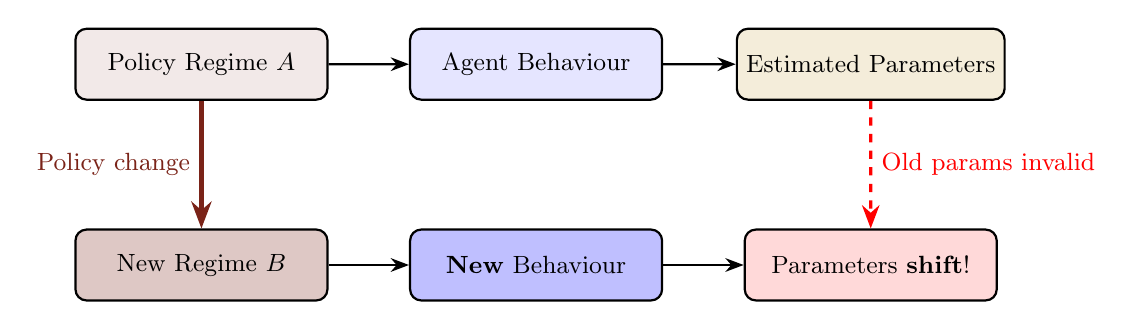
\begin{tikzpicture}[>=Stealth, thick, scale=0.85,
  box/.style={draw, rounded corners, minimum width=3.2cm, minimum height=0.9cm,
              font=\small, text centered}]
  \node[box, fill=UoERed!10] (regime) at (0,3) {Policy Regime $A$};
  \node[box, fill=blue!10] (behaviour) at (5,3) {Agent Behaviour};
  \node[box, fill=UoEGold!15] (params) at (10,3) {Estimated Parameters};

  \node[box, fill=UoERed!25] (regime2) at (0,0) {New Regime $B$};
  \node[box, fill=blue!25] (behaviour2) at (5,0) {\textbf{New} Behaviour};
  \node[box, fill=red!15] (params2) at (10,0) {Parameters \textbf{shift}!};

  \draw[->] (regime) -- (behaviour);
  \draw[->] (behaviour) -- (params);
  \draw[->, UoERed, line width=1.5pt] (regime) -- node[left, font=\small] {Policy change} (regime2);
  \draw[->] (regime2) -- (behaviour2);
  \draw[->] (behaviour2) -- (params2);
  \draw[->, red, dashed, line width=1.2pt] (params) -- node[right, font=\small, text=red]
    {Old params invalid} (params2);
\end{tikzpicture}
\end{center}
\vspace{0.5em}
This forced a methodological revolution toward \textbf{microfounded models}
(DSGE) whose deep parameters (preferences, technology) remain invariant
to policy changes.
\end{frame}

\begin{frame}{The Volcker Disinflation}
\begin{columns}[T]
\column{0.55\textwidth}
\begin{itemize}
  \item 1979: \textbf{Paul Volcker} appointed Fed Chairman.
  \item Abandoned interest-rate targeting; targeted monetary aggregates.
  \item Deliberately induced severe recession to break inflation expectations.
  \item Unemployment peaked above 10\%.
  \item Inflation fell from double digits to $\approx4\%$ by 1983.
\end{itemize}
\vspace{0.3em}
Demonstrated both the \textbf{power of expectations} (once credibly
anchored, inflation fell) and the \alert{cost of re-anchoring} them.
\column{0.4\textwidth}
\begin{center}
\begin{tikzpicture}[scale=0.55, >=Stealth]
  \draw[->] (0,0) -- (8,0) node[below, font=\scriptsize] {Year};
  \draw[->] (0,0) -- (0,7) node[left, font=\scriptsize] {$\pi$ (\%)};
  \draw[thick, UoERed] plot[smooth] coordinates
    {(0.5,6) (1.5,6.5) (2.5,5.8) (3.5,2.5) (4.5,1.8) (5.5,2) (6.5,2.2)};
  \draw[dashed, gray] (0,2) -- (7,2);
  \node[left, font=\tiny] at (0,2) {Target};
  \node[below, font=\tiny] at (0.5,0) {'78};
  \node[below, font=\tiny] at (3.5,0) {'82};
  \node[below, font=\tiny] at (6.5,0) {'86};
  \draw[->, thick, UoEGold] (2.7,5.5) -- (3.3,3) node[midway, right, font=\tiny] {Volcker};
\end{tikzpicture}
\end{center}
\vspace{0.2em}
{\scriptsize Stylised US inflation path, 1978--1986.}
\end{columns}
\end{frame}

\begin{frame}{Edinburgh Connection}
\begin{block}{Theory and Empirics Meet}
The University of Edinburgh's tradition --- from David Hume's monetary theory
to modern theoretical and applied econometrics --- is precisely the
synthesis the expectations revolution demanded.
\end{block}
\vspace{0.5em}
\begin{itemize}
  \item The debate was never purely theoretical --- driven by
        \textbf{empirical failures} (breakdown of the Phillips curve).
  \item Never purely empirical --- required \textbf{deep theoretical innovation}
        (rational expectations, the Lucas critique).
  \item Edinburgh trains economists who move fluently between formal theory,
        computational modelling, and careful empirical work --- exactly
        the skill set the expectations revolution required.
\end{itemize}
\end{frame}

\begin{frame}{Timeline: The Expectations Revolution}
\begin{center}
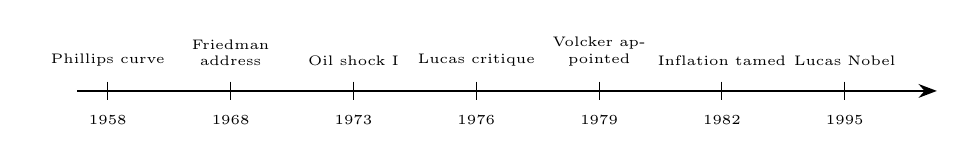
\begin{tikzpicture}[>=Stealth, scale=0.78]
  % Timeline
  \draw[thick, ->] (0,0) -- (14,0);
  % Events
  \foreach \x/\yr/\evt in {
    0.5/1958/{Phillips curve},
    2.5/1968/{Friedman address},
    4.5/1973/{Oil shock I},
    6.5/1976/{Lucas critique},
    8.5/1979/{Volcker appointed},
    10.5/1982/{Inflation tamed},
    12.5/1995/{Lucas Nobel}} {
    \draw (\x,0.15) -- (\x,-0.15);
    \node[below, font=\tiny, text width=1.6cm, align=center] at (\x,-0.25) {\yr};
    \node[above, font=\tiny, text width=1.8cm, align=center] at (\x,0.25) {\evt};
  }
\end{tikzpicture}
\end{center}
\vspace{0.5em}
From stable trade-off to intellectual revolution in under two decades.\\[4pt]
The lesson: \textbf{people are not passive objects of policy.}
They think, anticipate, and adapt.
\end{frame}

% -------------------------------------------------------------
\section{Part II --- The Computation}
% -------------------------------------------------------------

\begin{frame}[fragile]{Setting Up}
\begin{lstlisting}
import numpy as np
import matplotlib.pyplot as plt

# Reproducibility
np.random.seed(42)
\end{lstlisting}
\vspace{0.5em}
\begin{itemize}
  \item \texttt{numpy} --- numerical arrays, random number generation
  \item \texttt{matplotlib} --- plotting
  \item We will simulate inflation processes, expectation formation,
        and policy experiments
\end{itemize}
\end{frame}

\begin{frame}{The Original Phillips Curve}
The naive Phillips curve posits a simple inverse relationship:
\[
  \pi = \alpha - \beta\,(u - u^*)
\]
where $u^*$ is the natural rate of unemployment.
\vspace{0.5em}
\begin{columns}[T]
\column{0.48\textwidth}
\begin{block}{Parameters}
  $\alpha = 3.0$ (baseline inflation at $u = u^*$)\\
  $\beta = 1.2$ (slope)\\
  $u^* = 5.0\%$ (natural rate)
\end{block}
\column{0.48\textwidth}
\begin{block}{Interpretation}
  At $u = 3\%$: $\pi = 3 + 1.2(2) = 5.4\%$\\
  At $u = 7\%$: $\pi = 3 - 1.2(2) = 0.6\%$\\
  The ``menu of options''
\end{block}
\end{columns}
\end{frame}

\begin{frame}{The AR(1) Process for Inflation}
Inflation is often modelled as a first-order autoregressive process:
\[
  \pi_t = a + \rho\,\pi_{t-1} + \varepsilon_t, \qquad
  \varepsilon_t \sim N(0, \sigma^2)
\]
\vspace{0.3em}
\begin{columns}[T]
\column{0.48\textwidth}
\textbf{Key properties} (when $|\rho| < 1$):
\begin{itemize}
  \item Stationary
  \item Unconditional mean: $\mu = \dfrac{a}{1 - \rho}$
  \item Unconditional variance: $\sigma^2_\pi = \dfrac{\sigma^2}{1 - \rho^2}$
  \item Autocorrelation at lag $k$: $\rho^k$
\end{itemize}
\column{0.48\textwidth}
\textbf{Special cases:}
\begin{itemize}
  \item $\rho = 0$: white noise
  \item $\rho = 1$: random walk (non-stationary)
  \item $|\rho| > 1$: explosive
  \item High $\rho$: persistent, slow mean-reversion
\end{itemize}
\end{columns}
\end{frame}

\begin{frame}[fragile]{Simulating an AR(1) Process}
\begin{lstlisting}
def simulate_ar1(a, rho, sigma, T, pi_0=None):
    """Simulate AR(1): pi_t = a + rho * pi_{t-1} + eps_t."""
    if pi_0 is None:
        pi_0 = a / (1 - rho) if abs(rho) < 1 else 0.0
    pi = np.zeros(T)
    pi[0] = pi_0
    eps = np.random.normal(0, sigma, T)
    for t in range(1, T):
        pi[t] = a + rho * pi[t-1] + eps[t]
    return pi

# Parameters
T = 200; a = 0.5; rho = 0.85; sigma = 0.5
pi_ar1 = simulate_ar1(a, rho, sigma, T)

# Theoretical moments
mu_theory = a / (1 - rho)    # = 3.333
var_theory = sigma**2 / (1 - rho**2)  # = 0.948
\end{lstlisting}
\end{frame}

\begin{frame}{Adaptive Expectations}
Under \textbf{adaptive expectations}, agents look \textit{backward}:
\[
  \pi^e_t = \pi_{t-1}
\]

\vspace{0.3em}
\begin{itemize}
  \item Simple rule: expect tomorrow's inflation to equal today's.
  \item When inflation is rising, adaptive expectations systematically
        \alert{underpredict}.
  \item When inflation is falling, they systematically \alert{overpredict}.
  \item Forecast errors are \textbf{serially correlated} --- a rational
        agent should be able to do better.
\end{itemize}

\vspace{0.5em}
\begin{alertblock}{Key Weakness}
Adaptive expectations leave \textbf{money on the table}:
predictable patterns in forecast errors mean the agent is not using
all available information.
\end{alertblock}
\end{frame}

\begin{frame}[fragile]{Adaptive Expectations: Code}
\begin{lstlisting}
pi_actual = pi_ar1.copy()

# Adaptive: expected = last period's actual
pi_e_adaptive = np.zeros(T)
pi_e_adaptive[0] = pi_actual[0]
for t in range(1, T):
    pi_e_adaptive[t] = pi_actual[t - 1]

# Forecast errors
fe_adaptive = pi_actual - pi_e_adaptive

print(f"Mean forecast error:  {fe_adaptive.mean():.4f}")
print(f"Std forecast error:   {fe_adaptive.std():.4f}")
\end{lstlisting}
\vspace{0.3em}
The adaptive forecast tracks the actual series but with a \textbf{lag} ---
always one step behind any systematic trend.
\end{frame}

\begin{frame}{Rational Expectations}
Under \textbf{rational expectations}, agents use \textit{all available information}:
\[
  \pi^e_t = E[\pi_t \mid \mathcal{I}_{t-1}]
\]

If inflation follows $\pi_t = a + \rho\,\pi_{t-1} + \varepsilon_t$ and
agents know $a$, $\rho$, and observe $\pi_{t-1}$:
\[
  \pi^e_t = a + \rho\,\pi_{t-1}
\]

\vspace{0.3em}
\begin{itemize}
  \item Forecast error: $\pi_t - \pi^e_t = \varepsilon_t$ --- pure white noise.
  \item \textbf{Mean-zero} and \textbf{serially uncorrelated}.
  \item No information at time $t-1$ can improve the forecast.
\end{itemize}

\vspace{0.3em}
\begin{block}{Not Clairvoyance}
Rational expectations $\neq$ perfect foresight. Agents make errors,
but the errors are \textbf{unpredictable}. No systematic pattern
remains to exploit.
\end{block}
\end{frame}

\begin{frame}[fragile]{Rational Expectations: Code}
\begin{lstlisting}
# Rational: conditional expectation of AR(1)
pi_e_rational = np.zeros(T)
pi_e_rational[0] = mu_theory  # unconditional mean
for t in range(1, T):
    pi_e_rational[t] = a + rho * pi_actual[t - 1]

# Forecast errors
fe_rational = pi_actual - pi_e_rational

print(f"Mean forecast error:  {fe_rational.mean():.4f}")
print(f"Std forecast error:   {fe_rational.std():.4f}")

# Serial correlation of errors
from numpy import corrcoef
ac_adapt = corrcoef(fe_adaptive[1:], fe_adaptive[:-1])[0,1]
ac_ratio = corrcoef(fe_rational[1:], fe_rational[:-1])[0,1]
print(f"Autocorr (adaptive):  {ac_adapt:.4f}")   # high
print(f"Autocorr (rational):  {ac_ratio:.4f}")   # near zero
\end{lstlisting}
\end{frame}

\begin{frame}{Comparing Forecast Errors}
\begin{center}
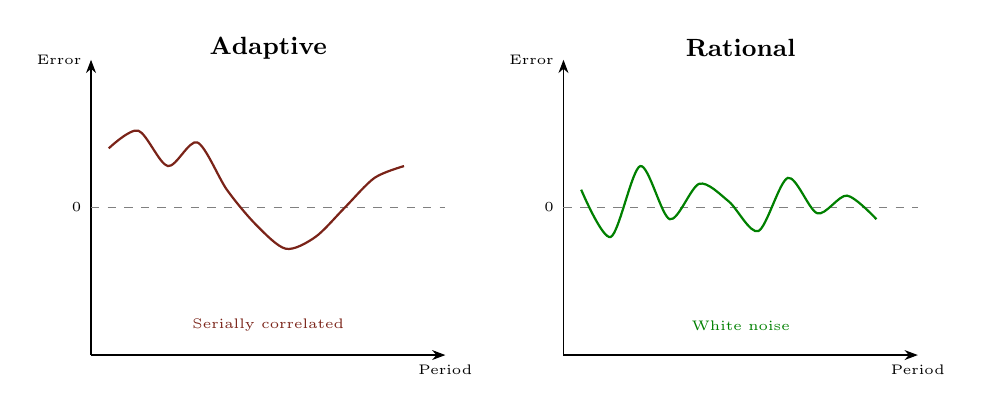
\begin{tikzpicture}[scale=0.75, >=Stealth]
  % Adaptive panel
  \node[font=\small\bfseries] at (3,5.2) {Adaptive};
  \draw[->] (0,0) -- (6,0) node[below, font=\tiny] {Period};
  \draw[->] (0,0) -- (0,5) node[left, font=\tiny] {Error};
  \draw[dashed, gray] (0,2.5) -- (6,2.5);
  \node[left, font=\tiny] at (0,2.5) {$0$};
  % Serially correlated errors
  \draw[thick, UoERed] plot[smooth] coordinates
    {(0.3,3.5) (0.8,3.8) (1.3,3.2) (1.8,3.6) (2.3,2.8) (2.8,2.2)
     (3.3,1.8) (3.8,2.0) (4.3,2.5) (4.8,3.0) (5.3,3.2)};
  \node[UoERed, font=\tiny] at (3,0.5) {Serially correlated};

  % Rational panel
  \begin{scope}[xshift=8cm]
  \node[font=\small\bfseries] at (3,5.2) {Rational};
  \draw[->] (0,0) -- (6,0) node[below, font=\tiny] {Period};
  \draw[->] (0,0) -- (0,5) node[left, font=\tiny] {Error};
  \draw[dashed, gray] (0,2.5) -- (6,2.5);
  \node[left, font=\tiny] at (0,2.5) {$0$};
  % White noise errors
  \draw[thick, green!50!black] plot[smooth] coordinates
    {(0.3,2.8) (0.8,2.0) (1.3,3.2) (1.8,2.3) (2.3,2.9) (2.8,2.6)
     (3.3,2.1) (3.8,3.0) (4.3,2.4) (4.8,2.7) (5.3,2.3)};
  \node[green!50!black, font=\tiny] at (3,0.5) {White noise};
  \end{scope}
\end{tikzpicture}
\end{center}
\vspace{0.3em}
\begin{columns}[T]
\column{0.48\textwidth}
\textbf{Adaptive:} Errors show patterns.\\
A rational agent could exploit them.
\column{0.48\textwidth}
\textbf{Rational:} Errors are unpredictable.\\
No further improvement possible.
\end{columns}
\end{frame}

\begin{frame}{The Policy Experiment}
The heart of the matter: can the government \alert{exploit the Phillips curve}?
\vspace{0.3em}

\textbf{Expectations-augmented Phillips curve:}
\[
  \pi_t = \pi^e_t - \beta\,(u_t - u^*) + \varepsilon_t
\]
\textbf{Policy rule:} after period 10, government injects extra inflation
$\delta = 2$ percentage points per period.
\vspace{0.3em}
\begin{columns}[T]
\column{0.48\textwidth}
\begin{block}{Under Adaptive}
$\pi^e_t = \pi_{t-1}$. The surprise
$\pi_t - \pi^e_t = \delta + \varepsilon_t > 0$
pushes $u_t < u^*$. But inflation
\textbf{ratchets up} each period.
\end{block}
\column{0.48\textwidth}
\begin{block}{Under Rational}
Agents \textit{know} the policy rule:
$\pi^e_t = \pi_{t-1} + \delta$.
Surprise $= \varepsilon_t$ only.
$u_t = u^* + \text{noise}$.
\textbf{No real effect.}
\end{block}
\end{columns}
\end{frame}

\begin{frame}[fragile]{Policy Experiment: Code}
\begin{lstlisting}
T_pol = 60; u_nat = 5.0; beta_pc = 1.0; delta = 2.0
policy_start = 10
eps = np.random.normal(0, 0.3, T_pol)

# --- Adaptive ---
pi_a, pi_e_a, u_a = np.zeros(T_pol), np.zeros(T_pol), np.full(T_pol, u_nat)
pi_a[0] = pi_e_a[0] = 2.0
for t in range(1, T_pol):
    pi_e_a[t] = pi_a[t-1]
    pi_a[t] = pi_e_a[t] + (delta if t>=policy_start else 0) + eps[t]
    u_a[t] = u_nat - (pi_a[t] - pi_e_a[t] - eps[t]) / beta_pc

# --- Rational ---
pi_r, pi_e_r, u_r = np.zeros(T_pol), np.zeros(T_pol), np.full(T_pol, u_nat)
pi_r[0] = pi_e_r[0] = 2.0
for t in range(1, T_pol):
    pi_e_r[t] = pi_r[t-1] + (delta if t>=policy_start else 0)
    pi_r[t] = pi_e_r[t] + eps[t]
    u_r[t] = u_nat - (pi_r[t] - pi_e_r[t] - eps[t]) / beta_pc
\end{lstlisting}
\end{frame}

\begin{frame}{Policy Experiment: Results}
\begin{center}
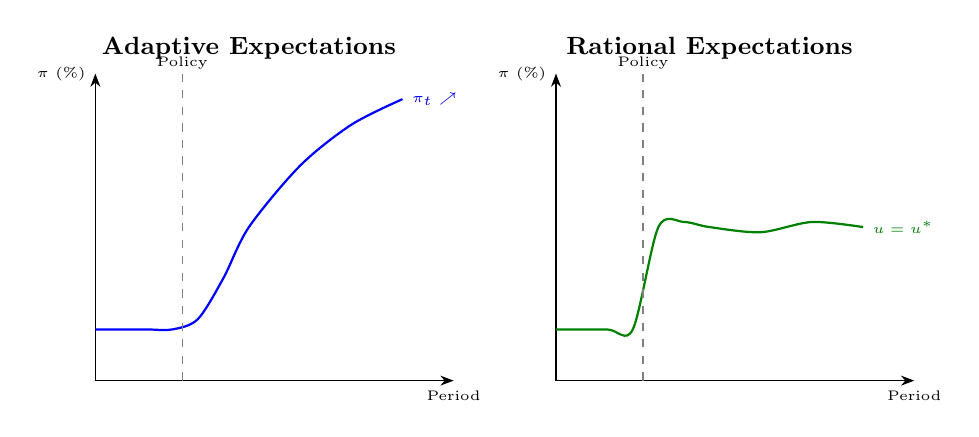
\begin{tikzpicture}[scale=0.65, >=Stealth]
  % Adaptive panel
  \node[font=\small\bfseries] at (3,6.5) {Adaptive Expectations};
  \draw[->] (0,0) -- (7,0) node[below, font=\tiny] {Period};
  \draw[->] (0,0) -- (0,6) node[left, font=\tiny] {$\pi$ (\%)};
  % Inflation ratchets up
  \draw[thick, blue] plot[smooth] coordinates
    {(0,1) (1,1) (1.5,1) (2,1.2) (2.5,2) (3,3) (4,4.2) (5,5) (6,5.5)};
  \draw[dashed, black!50] (1.7,0) -- (1.7,6);
  \node[font=\tiny] at (1.7,6.2) {Policy};
  \node[blue, font=\tiny, right] at (6,5.5) {$\pi_t \nearrow$};

  % Rational panel
  \begin{scope}[xshift=9cm]
  \node[font=\small\bfseries] at (3,6.5) {Rational Expectations};
  \draw[->] (0,0) -- (7,0) node[below, font=\tiny] {Period};
  \draw[->] (0,0) -- (0,6) node[left, font=\tiny] {$\pi$ (\%)};
  % Inflation jumps to new level
  \draw[thick, green!50!black] plot[smooth] coordinates
    {(0,1) (1,1) (1.5,1) (2,3) (2.5,3.1) (3,3) (4,2.9) (5,3.1) (6,3)};
  \draw[dashed, black!50] (1.7,0) -- (1.7,6);
  \node[font=\tiny] at (1.7,6.2) {Policy};
  \node[green!50!black, font=\tiny, right] at (6,3) {$u = u^*$};
  \end{scope}
\end{tikzpicture}
\end{center}
\vspace{0.3em}
\begin{itemize}
  \item \textbf{Adaptive}: unemployment drops temporarily, but inflation
        \alert{accelerates} without bound. Friedman's prediction.
  \item \textbf{Rational}: unemployment stays at $u^*$. Policy only raises
        inflation. Lucas's result.
\end{itemize}
\end{frame}

\begin{frame}{The Augmented Phillips Curve}
\begin{center}
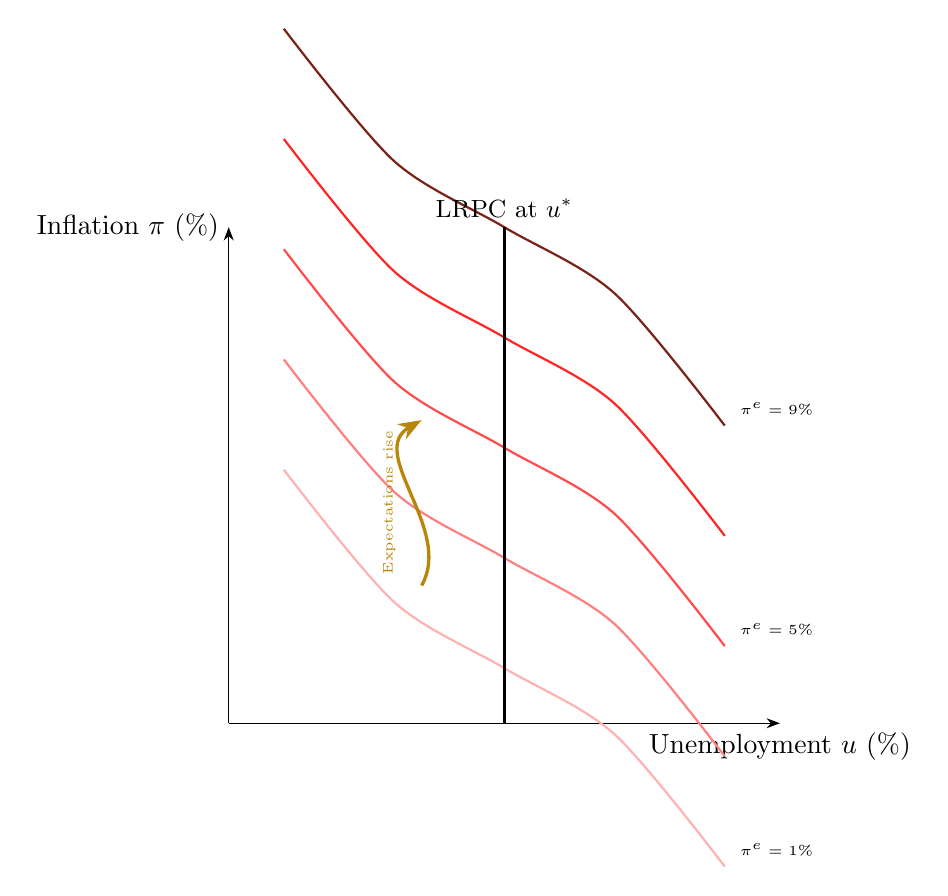
\begin{tikzpicture}[scale=0.7, >=Stealth]
  % Axes
  \draw[->] (0,0) -- (10,0) node[below] {Unemployment $u$ (\%)};
  \draw[->] (0,0) -- (0,9) node[left] {Inflation $\pi$ (\%)};

  % Short-run Phillips curves at different pi^e levels
  \foreach \pe/\col/\lab in {1/red!30/1, 3/red!50/3, 5/red!70/5, 7/red!85/7, 9/UoERed/9} {
    \draw[thick, \col] plot[smooth] coordinates
      {(1,{\pe+3.6}) (3,{\pe+1.2}) (5,\pe) (7,{\pe-1.2}) (9,{\pe-3.6})};
  }
  % Labels for selected curves
  \node[font=\tiny, right] at (9.1,{1-3.6+0.3}) {$\pi^e = 1\%$};
  \node[font=\tiny, right] at (9.1,{5-3.6+0.3}) {$\pi^e = 5\%$};
  \node[font=\tiny, right] at (9.1,{9-3.6+0.3}) {$\pi^e = 9\%$};

  % Long-run vertical line
  \draw[very thick, black] (5,0) -- (5,9);
  \node[above, font=\small] at (5,9) {LRPC at $u^*$};

  % Arrow showing shift
  \draw[->, UoEGold, very thick] (3.5,2.5) to[out=60,in=210] (3.5,5.5);
  \node[UoEGold, font=\tiny, left] at (3.2,4) {\rotatebox{90}{Expectations rise}};
\end{tikzpicture}
\end{center}
\vspace{0.3em}
Each short-run curve is conditioned on $\pi^e$. Expanding demand
moves along one curve, but \textbf{shifts the whole curve up}.
The long-run Phillips curve is \alert{vertical}.
\end{frame}

% -------------------------------------------------------------
\section{Part III --- Exercises \& Discussion}
% -------------------------------------------------------------

\begin{frame}{Exercise 1: AR(1) Persistence and Stationarity}
Explore how the persistence parameter $\rho$ shapes an AR(1) process.
\vspace{0.3em}
\begin{enumerate}
  \item Simulate four AR(1) processes ($T = 300$, $a = 0.5$, $\sigma = 0.5$) with\\
        $\rho \in \{0.2,\; 0.7,\; 0.95,\; 1.0\}$. Use $\pi_0 = 0$.
        Plot on a $2 \times 2$ grid.
  \item For stationary cases, compare theoretical and sample moments:\\
        $\mu = a/(1-\rho)$, \; $\sigma_\pi = \sigma/\sqrt{1-\rho^2}$.
  \item Compute sample autocorrelation at lags $k = 1, \ldots, 20$.\\
        Compare with theoretical $\rho^k$.
  \item Why is $\rho = 1$ non-stationary? When might inflation have a unit root?
\end{enumerate}
\vspace{0.3em}
\begin{alertblock}{Key Insight}
High $\rho$ means shocks are persistent; $\rho = 1$ means shocks
are \textbf{permanent}. Credible monetary policy makes inflation stationary.
\end{alertblock}
\end{frame}

\begin{frame}[fragile]{Exercise 1: Starter Code}
\begin{lstlisting}
T_ex1 = 300; a_ex1 = 0.5; sigma_ex1 = 0.5
rhos = [0.2, 0.7, 0.95, 1.0]
np.random.seed(2024)

fig, axes = plt.subplots(2, 2, figsize=(14, 8), sharex=True)
axes = axes.flatten()

for i, rho_i in enumerate(rhos):
    pi_i = simulate_ar1(a_ex1, rho_i, sigma_ex1, T_ex1, pi_0=0.0)
    axes[i].plot(pi_i, linewidth=0.8)
    axes[i].set_title(f'$\\rho = {rho_i}$')
    if rho_i < 1:
        mu_i = a_ex1 / (1 - rho_i)
        axes[i].axhline(y=mu_i, color='red', linestyle='--',
                        label=f'$\\mu = {mu_i:.2f}$')
        axes[i].legend()

plt.tight_layout()
plt.show()
\end{lstlisting}
\end{frame}

\begin{frame}{Exercise 2: The Lucas Critique in Action}
A central bank sets inflation via a policy rule:
\[
  \pi_t = \bar{\pi} + \gamma\,(u_{t-1} - u^*)
\]
with $\bar{\pi} = 2\%$, $\gamma = -0.8$, $u^* = 5\%$.
Unemployment obeys:
\[
  u_t = u^* - \alpha_{pc}\,(\pi_t - \pi^e_t) + \eta_t
\]
\vspace{0.3em}
\begin{enumerate}
  \item[(a)] Simulate under \textbf{adaptive} expectations ($\pi^e_t = \pi_{t-1}$).
  \item[(b)] Simulate under \textbf{rational} expectations
        ($\pi^e_t = \bar{\pi} + \gamma(u_{t-1} - u^*)$).\\
        Show that $\pi_t - \pi^e_t = 0$ $\Rightarrow$ no systematic effect.
  \item[(c)] Change the policy to $\gamma = -1.6$. Compare outcomes.
  \item[(d)] Explain: why can an econometrician not use estimates from (a)
        to predict (c)?
\end{enumerate}
\end{frame}

\begin{frame}[fragile]{Exercise 2: Starter Code}
\begin{lstlisting}
def simulate_lucas_critique(gamma, exp_type='adaptive',
                            T=100, seed=99):
    np.random.seed(seed)
    eta = np.random.normal(0, 0.3, T)
    pi = np.zeros(T); pi_e = np.zeros(T)
    u = np.full(T, 5.0)
    pi[0] = pi_e[0] = 2.0; u[0] = 5.0 + eta[0]
    for t in range(1, T):
        pi[t] = 2.0 + gamma * (u[t-1] - 5.0)
        if exp_type == 'adaptive':
            pi_e[t] = pi[t - 1]
        else:  # rational
            pi_e[t] = 2.0 + gamma * (u[t-1] - 5.0)
        u[t] = 5.0 - 0.5 * (pi[t] - pi_e[t]) + eta[t]
    return pi, pi_e, u

pi_a, _, u_a = simulate_lucas_critique(-0.8, 'adaptive')
pi_r, _, u_r = simulate_lucas_critique(-0.8, 'rational')
\end{lstlisting}
\end{frame}

\begin{frame}{Exercise 3: Disinflation --- Cold Turkey vs.\ Gradualism}
A Volcker-style disinflation: reduce $\pi$ from $10\%$ to $2\%$.
\vspace{0.3em}
\begin{columns}[T]
\column{0.48\textwidth}
\begin{block}{Cold Turkey}
Immediately set $\pi_t = 2\%$ for all $t \geq 1$.\\
Fast but potentially very painful.
\end{block}
\column{0.48\textwidth}
\begin{block}{Gradualism}
Reduce inflation linearly over 20 periods:\\
$\pi_t = \max(2,\; 10 - 0.4t)$.\\
Slower, spread the cost.
\end{block}
\end{columns}
\vspace{0.3em}
\begin{enumerate}
  \item[(a)] Simulate both under \textbf{adaptive} expectations. Plot $\pi_t$ and $u_t$.
  \item[(b)] Repeat under \textbf{rational} expectations (full credibility).
  \item[(c)] Compute the \textbf{sacrifice ratio}: cumulative excess unemployment
        per percentage point of disinflation. Compare in a bar chart.
  \item[(d)] Why is disinflation costly under adaptive but costless under rational
        expectations? What does this say about \textbf{credibility}?
\end{enumerate}
\end{frame}

\begin{frame}[fragile]{Exercise 3: Starter Code}
\begin{lstlisting}
T_ex3 = 50; pi_0_ex3 = 10.0; pi_target = 2.0
np.random.seed(777)
eta = np.random.normal(0, 0.2, T_ex3)

def disinflation_path(strategy, T):
    pi_cb = np.zeros(T); pi_cb[0] = pi_0_ex3
    for t in range(1, T):
        if strategy == 'cold_turkey':
            pi_cb[t] = pi_target
        else:  # gradual
            pi_cb[t] = max(pi_target,
                           pi_0_ex3 - (pi_0_ex3-pi_target)*t/20)
    return pi_cb

def sacrifice_ratio(u, u_star=5.0):
    return np.sum(np.maximum(u - u_star, 0)) / (10 - 2)
\end{lstlisting}
\end{frame}

% -------------------------------------------------------------
\section{Key Takeaways}
% -------------------------------------------------------------

\begin{frame}{What We Learned This Week}
\begin{enumerate}
  \item The \textbf{naive Phillips curve} offered an apparent trade-off between
        inflation and unemployment, but it was an illusion.
  \item \textbf{Friedman} (1968) showed the trade-off is temporary: in the long run,
        the Phillips curve is \textit{vertical} at the natural rate.
  \item \textbf{Lucas} took this further with \textbf{rational expectations}:
        systematic policy has no real effect because agents anticipate it.
  \item The \textbf{Lucas critique} invalidated old-style econometric policy
        evaluation --- parameters shift when regimes change.
  \item \textbf{Credibility} is the crucial variable: disinflation is costly
        when expectations must be re-anchored, as the Volcker episode showed.
  \item We can \textbf{simulate} all of this: AR(1) processes, adaptive vs.\
        rational expectations, and policy experiments that demonstrate
        these ideas computationally.
\end{enumerate}
\end{frame}

\begin{frame}{Further Reading}
\begin{itemize}
  \item Friedman, M. ``The Role of Monetary Policy,''
        \textit{American Economic Review}, 1968.
  \item Lucas, R. ``Econometric Policy Evaluation: A Critique,''
        \textit{Carnegie-Rochester Conference Series}, 1976.
  \item Sargent, T. and N.~Wallace. ``Rational Expectations, the Optimal
        Monetary Instrument, and the Optimal Money Supply Rule,''
        \textit{Journal of Political Economy}, 1975.
  \item Mankiw, N.~G. \textit{Macroeconomics}, Chs.~14--15.
  \item Romer, D. \textit{Advanced Macroeconomics}, Ch.~6.
\end{itemize}
\vspace{1em}
\begin{center}
\textbf{Next week:} The New Keynesian Synthesis ---\\
rational expectations meets price rigidities,\\
and why credible institutions matter for monetary policy.
\end{center}
\end{frame}

\end{document}
